\documentclass[serif,mathserif,compress]{beamer}
\usepackage{amsmath, amsfonts, epsfig, xspace}
\usepackage{algorithm,algorithmic}
\usepackage{pstricks,pst-node}
\usepackage{multimedia}
\usepackage{listings}
\usepackage[normal,tight,center]{subfigure}
\setlength{\subfigcapskip}{-.5em}
\usepackage{beamerthemesplit}
%\usepackage{../beamerthemelankton-keynote}
%\usetheme{Warsaw}
%\useoutertheme[subsection=false]{smoothbars}
\usetheme{Madrid}
\useoutertheme[footline=authortitle,subsection=true]{miniframes}

\lstset{ %
basicstyle=\footnotesize,        % the size of the fonts that are used for the code
tabsize=2,	                     % sets default tabsize to 2 spaces
}

\begin{document}

\author[Joe Rocklin]{
\begin{tabular}[t]{c c}
  Joe Rocklin & Tom Rocklin \\
  joseph.rocklin@siemens.com &  tom.rocklin@siemens.com \\
  @joerocklin &
\end{tabular}
}

\title[Lesson 01\hspace{2em}\insertframenumber/\inserttotalframenumber]{Lesson 01 - What is Software}

\date{September 15, 2015} %leave out for today's date to be insterted

\institute{Siemens PLM Software}

\maketitle

\section{Introduction}  % add these to see outline in slides
\begin{frame}{Tom Rocklin}
  Tom Rocklin
  \begin{columns}[T]
  \begin{column}[T]{.5\textwidth}
    \begin{itemize}
    \item Univeristy of Cincinnati\\Mechanical Engineering
    \item SDRC Coop starting in 1972\\Mechanical Engineering Consulting
    \item Now doing Software Development
    \end{itemize}
  \end{column}
  \end{columns}
\end{frame}

\begin{frame}{Siemens}
  A brief history of how we got to where we are...
\end{frame}

\begin{frame}{Joe Rocklin}
  Joe Rocklin
  \begin{columns}[T]
  \begin{column}[T]{.5\textwidth}
    \begin{itemize}
    \item Milford HS, 2000
    \item Univeristy of Cincinnati\\B.S. Computer Science 2005
    \item University of Cincinnati\\Graduate studies in Computer Engineering
    \end{itemize}
  \end{column}
  \pause
  \begin{column}[T]{.5\textwidth}
    \begin{itemize}
    \item Co-Op at SDRC, MeadWestvaco, Cinergy, and UC Research
    \item Northrop Grumman, 2005-2012
    \item Siemens PLM, 2012-Present
    \item HTG, LLC 2006-Present
    \end{itemize}
  \end{column}
  \end{columns}
\end{frame}

\begin{frame}{Areas of Interest}
  \begin{itemize}
  \item Operating Systems
  \item Hardware/Software Interactions
  \item Distributed Systems
  \item Security
  \item Education
  \end{itemize}
\end{frame}

\begin{frame}{What it Software?}
  \begin{block}{Software is...}
    Software is a set of machine-readable instructions which directs a processor to perform specific actions.
  \end{block}
\end{frame}

\section{A Look at Hardware}

\begin{frame}{Processors}
  Three main tasks:
  \begin{itemize}
  \item<1-> Fetch \only<2->{ - Read an instruction from memory}
  \item<1-> Decode \only<3->{ - Figure out what the instruction is}
  \item<1-> Execute \only<4->{ - Do whatever the instruction says to do}
  \end{itemize}
\end{frame}

\begin{frame}{Memory}
  Memory Heirarchy
  \begin{itemize}
  \item<1-> Hard Drives \only<2->{ - Terrabytes or more}
  \item<3-> RAM \only<4->{ - 10's - 100's of Gigabytes}
  \item<5-> Cache\only<8->{\footnote{Based on Intel Skylake series processors, announced August 2015}} \only<6->{ - On the processor silcon directly}
    \begin{itemize}
    \item<7-> L3 \only<8->{ - 8192KiB shared}
    \item<7-> L2 \only<8->{ -  256KiB per core}
    \item<7-> L1 \only<8->{ -   64KiB per core, split between data and instruction}
    \end{itemize}
  \item<9-> Registers
  \end{itemize}
\end{frame}

\begin{frame}{Interconnections}
  \begin{figure}
  \centering
  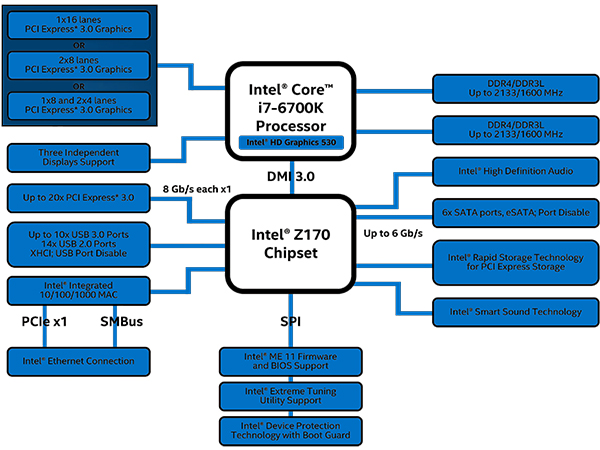
\includegraphics[height=0.7\textheight]{images/Intel-Z170-chipset-block-diagram.jpg}
  \caption{Intel Z170 Chipset Block Diagram}
  \label{fig:intel-z170-chipset}
  \end{figure}
\end{frame}

\section{Software}

\subsection{Instruction Sets}

\begin{frame}{Instruction Set}
  \begin{block}{}
    Every processor has a set of instructions which can be decoded and executed. These instructions map to the hardware which is available on the processor.
  \end{block}
\end{frame}

\begin{frame}{Types}
  \begin{columns}[T]
  \begin{column}[T]{.45\textwidth}
    \begin{block}{RISC}
      All processors have some basic instructions:
      \begin{itemize}
        \item Data handling and memory operations
        \item Arithmetic and logic operations
        \item Control flow operations
      \end{itemize}
    \end{block}
  \end{column}
  \pause
  \begin{column}[T]{.45\textwidth}
    \begin{block}{CISC}
      Processors with complex instruction sets may have dedicated hardware for:
      \begin{itemize}
        \item Moving chunks of data at once
        \item Complex mathematical operations (sine, cosine, square root, etc)
        \item Parallel operations
        \item Cryptographic functions
      \end{itemize}
    \end{block}
  \end{column}
  \end{columns}
\end{frame}

\begin{frame}{Machine Code}
  Let's say we want to add the value 5 to the value that is in the register called EAX:\\
  \pause

  \begin{block}{Machine Code}
    \begin{center}
    \begin{tabular}{|c|c|c|c|c|c|c|c|}
      \hline
      \multicolumn{8}{|c|}{01100110100000111100000000000101} \\
      \hline
      0110 & 0110 & 1000 & 0011 & 1100 & 0000 & 0000 & 0101 \\
      \hline
      6    & 6    & 8    & 3    & c    & 0    & 0    & 5 \\
      \hline
      \multicolumn{2}{|c}{66} & \multicolumn{2}{|c}{83} & \multicolumn{2}{|c}{c0} & \multicolumn{2}{|c|}{05} \\
      \hline
      \multicolumn{4}{|c}{Add a constant to a word} & \multicolumn{2}{|c}{EAX} & \multicolumn{2}{|c|}{5} \\
      \hline
    \end{tabular}
    \end{center}
  \end{block}

\end{frame}

\subsection{Assembly Language}
\begin{frame}[fragile]{Assembly Language}
  Writing the binary or hex can be done, but it's \emph{really} annoying.\\
  \pause
  Enter the Assembler
  \lstinputlisting[frame=none,language={[x86masm]Assembler}]{code/add.asm}
  \pause
  More assembler instructions can be found on
      \href{https://en.wikipedia.org/wiki/X86_instruction_listings}{Wikipedia}
      or on
      \href{http://www.intel.com/content/dam/www/public/us/en/documents/manuals/64-ia-32-architectures-software-developer-instruction-set-reference-manual-325383.pdf}{Intel's Website (pdf)}
\end{frame}

\begin{frame}[fragile]{Hello, World Assembler}
  \lstinputlisting[
    frame=none,
    language={[x86masm]Assembler},
    basicstyle=\tiny
    ]{code/hello_world.asm}
\end{frame}

\begin{frame}[fragile]{Hello, World Assembler Output}
  \begin{figure}
  \centering
  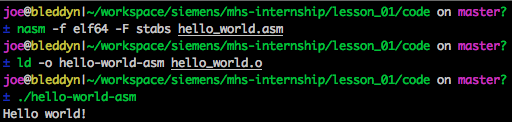
\includegraphics[width=\textwidth]{images/hello-world-asm.png}
  \caption{Hello World Assemble, Link, and Run}
  \label{fig:hello-world-asm-output}
  \end{figure}
\end{frame}

\subsection{High-Level Languages}

\begin{frame}{High-Level Languages}
  High-Level programming languages represent a wide array of options:
  \begin{itemize}[<+->]
    \item Compiled
    \begin{itemize}[<+->]
      \item Machine Code Generation - The syntax is compiled into the machine codes (C/C++, Fortran, Go, Rust)
      \item Intermediate Representation - The syntax is compiled into a representation which is interpreted by another program (Java, Erlang)
    \end{itemize}
    \item Interpreted - The syntax is evaluated, unchanged, by anther program (Python, Ruby, Javascript, PHP)
    \item Transpiled - The syntax is compiled into another syntax, which may then be compiled or interpreted (Opal, 6to5, HipHop)
  \end{itemize}
\end{frame}

\subsubsection{Compiled: C}
\begin{frame}[fragile]{Hello, World C}
  \lstinputlisting[
    frame=none,
    language={C},
    basicstyle=\tiny
    ]{code/hello_world.c}
  \pause

  \begin{figure}
  \centering
  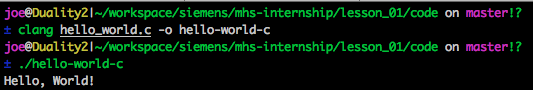
\includegraphics[width=\textwidth]{images/hello-world-c.png}
  \caption{Hello World C, Compile, and Run}
  \label{fig:hello-world-c-output}
  \end{figure}
\end{frame}


\subsubsection{Interpreted: Ruby}
\begin{frame}[fragile]{Hello, World Ruby}
  \lstinputlisting[
    frame=none,
    language={C},
    basicstyle=\tiny
    ]{code/hello_world.rb}
  \pause

  \begin{figure}
  \centering
  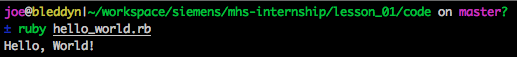
\includegraphics[width=\textwidth]{images/hello-world-ruby.png}
  \caption{Hello World Ruby, Compile, and Run}
  \label{fig:hello-world-ruby-output}
  \end{figure}
\end{frame}

\begin{frame}{More Hello World Examples}
  \begin{center}
    There are hundreds more examples at: \\
    \url{http://rosettacode.org/wiki/Hello_world}
  \end{center}
\end{frame}

\section{Wrap-up}

\begin{frame}{Wrapping Up}
  \begin{itemize}
    \item Software is just a series of instructions\\Computers are dumb, they just do what we tell them.
    \item Software comes in many different types and styles\\Each has its strengths and weaknesses
  \end{itemize}
\end{frame}

\begin{frame}{Questions}
\end{frame}

\begin{frame}{Before we meet again}
  Learn something about a programming language you know nothing about
  \begin{itemize}
    \item Use wikipedia, \url{https://en.wikipedia.org/wiki/Portal:Computer_programming} is a good place to start.
    \item What type of language is it (Low vs. High, compiled vs interpreted)?
    \item Are there big projects or compabies using it?
    \item Is there something that makes the language unique? Why would people chose the language?
  \end{itemize}
\end{frame}

\begin{frame}{Next Time}
  \begin{itemize}
    \item This little thing called The Internet
    \item More about types of software
  \end{itemize}
\end{frame}

\end{document}
